
In spline interpolation\cite{Boor1981}, the points are linked by a piecewise
polynomial.
The main advantage of using splines of order $p$, i.e., using polynomials of
order $p$ in the different intervals, is that we will not only obtain continuous
functions, as in the linear case, but we will also obtain functions
$\mathcal{C}^{p-1}[a,b]$, i.e., that are continuous and have $p-1$ continuous
derivatives. This fact is crucial in FDA, because we will need
to use derivatives in many parts of the analysis.

\begin{figure}[Example of spline interpolation]{FIG:SPLINE}{Example of spline interpolation}
	\subfigure[SBFIG:SPLINE1]{Spline interpolation}{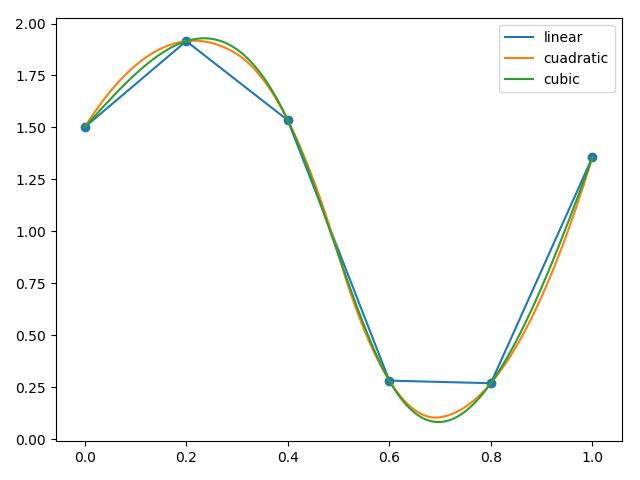
\includegraphics[width=7.5cm]{spline-interpolation}} \quad
	\subfigure[SBFIG:SPLINE2]{First derivatives}{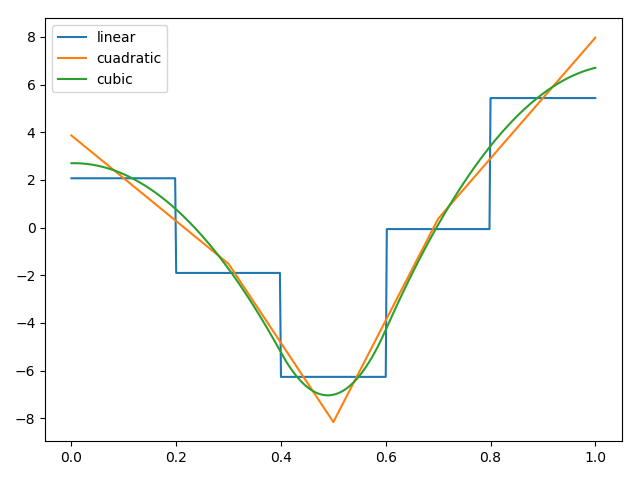
\includegraphics[width=7.5cm]{spline-derivatives-interpolation}}
\end{figure}

To achieve this, we have to match the values of the derivatives of the
adjacent splines in the interpolation knots. If we denote by
$s_k(t)=\sum_{j=0}^n c_{jk} t^k$ to the spline defined in the region
$[t_{k-1}, t_{k}]$, during the calculation of the coefficients $c_{jk}$, we must
impose the restriction $s_{k}^{(d)}(t_k) = s_{k+1}^{(d)}$ for \\ $d=1, \dots, p-1$.
For this purpose, we will define a linear system of equations which can be
solved iteratively. Figure \ref{SBFIG:SPLINE1} shows the result of interpolate a
temporal series using splines of different orders, and the first derivatives of
these splines, which are splines of order $p-1$ due to the derivation of the
polynomials.

\begin{figure}[Interpolation of surface]{FIG:BISPLINE}{Interpolation of surface with bicubic splines}
	\subfigure[SBFIG:BISPLINE1]{Surface interpolated}{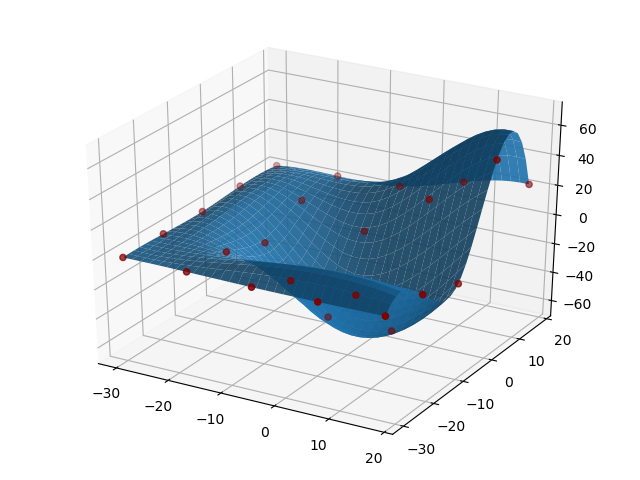
\includegraphics[width=7.5cm]{surface-bicubic}} \quad
	\subfigure[SBFIG:BISPLINE2]{Partial derivative $\partial_x$}{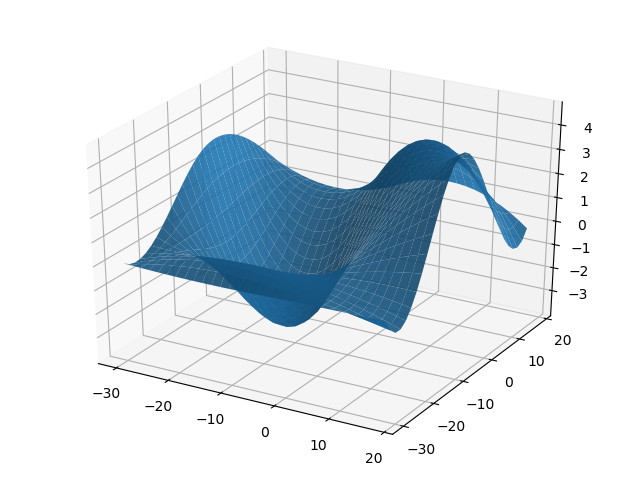
\includegraphics[width=7.5cm]{surface-bicubic-dx}}
\end{figure}

We can extend spline interpolation for multivariate functions, such as surfaces,
where bivariate splines will be used. In this case, triangulation is used
to calculate the regions in which the polynomials are defined. These polynomials
are of the form $s(x, y) = \sum_{0 \le i + j \le n} c_{i,j}x^i y^j$.
In the figure \ref{SBFIG:BISPLINE1} it is shown the result of the
interpolation of a surface using bicubic splines and the partial derivative
respect to its first parameter.
